% File: basic_elements.tex
\documentclass{standalone}
\usepackage{pgfplots}
\pgfplotsset{compat=1.18}
\usepackage[american]{circuitikz}
\usepackage{cmbright}

\definecolor{myred}{RGB}{170,0,0}
\definecolor{myblue}{RGB}{0,0,220}

\ctikzset{bipoles/resistor/height=0.2}
\ctikzset{bipoles/resistor/width=0.5}


\begin{document}
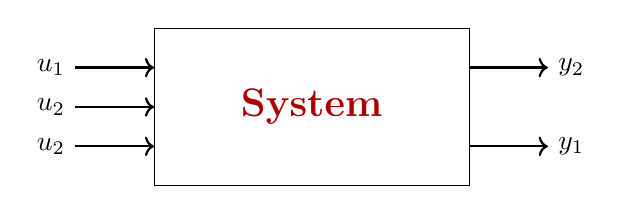
\begin{tikzpicture}
    % Rectangle for the system block
    \draw[black] (0,0) rectangle (4,2);
    \node[myred] at (2,1) {\Large \textbf{System}};
    % Input arrows
    \draw[->, thick] (-1, 1.5) node[anchor=east] {$u_1$} -- (0,1.5) ;
    \draw[->, thick] (-1, 1) node[anchor=east] {$u_2$} -- (0,1) ;
    \draw[->, thick] (-1, 0.5) node[anchor=east] {$u_2$} -- (0,0.5) ;
    % Output arrows
    \draw[->, thick] (4, 0.5) -- (5, 0.5) node[anchor=west] {$y_1$};
    \draw[->, thick] (4, 1.5) -- (5, 1.5) node[anchor=west] {$y_2$};
\end{tikzpicture}
\end{document}